\chapter{Project description}
\textit{This chapter seeks to explain the design and implementation of the project along with the tests used for improving the system.}
\section{Architecture}
The system consist of the CDU and a number of sensor nodes. This is seen on figure \ref{fig:systembdd}. Every sensor is powered by the custom power line communication bus. All communication is transmitted via the same bus. As figure \ref{fig:systembdd} shows the sensors are connected in a chain with a single wire. This means communication have to be carried by the power line. 
\begin{figure}[H]
	\centering
	\includegraphics[width=.9\textwidth]{billeder/11ProjectDescription/systembdd}
	\caption{System overview}
	\label{fig:systembdd}
\end{figure}
The bus is the central part of this chapter. It consists of several layers as displayed on figure \ref{fig:systemlayers}. The design of the protocol layer is found in the architecture document. The design of the subsequent layers can be found in the design and implementation document.
\begin{figure}[H]
	\centering
	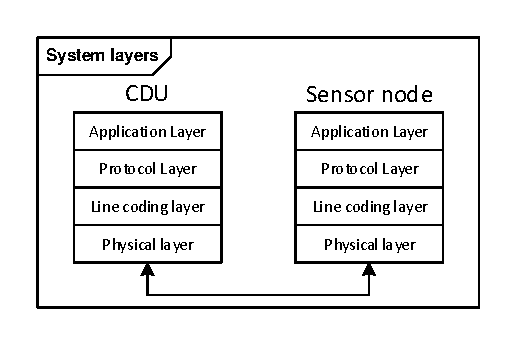
\includegraphics[width=.6\textwidth]{billeder/11ProjectDescription/System_Layers}
	\caption{System Layers}
	\label{fig:systemlayers}
\end{figure}
The protocol was designed with respects to already known protocols such as Modbus and I$^{2}$C. The principle of a start code and addressing was inspired by I$^{2}$C while the idea of function codes was inspired by Modbus. A data length multiplier tells the receiver how many bytes of data that are in the full message. A CRC check in the end ensures that the message was received correctly. This is further explained by table \ref{table:stdmsgtosensor}.
\begin{table}[H]
\centering
\begin{tabular}{|l|l|l|l|l|l|}
	\hline
	Start Sequence & Address & Function Code & DLM & Data & CRC  \\ \hline
	1 nibble & 1 nibble	& 1 nibble & 1 nibble & n bytes & 1 byte\\
	\hline
\end{tabular}
\caption{Message format for writing and reading}
\label{table:stdmsgtosensor}
\end{table}


\section{Design and implementation}
\textbf{Line Coding layer "design"}.\\
\fixme{Husk at slette.}
Hest

\textbf{Physical layer "design"}.\\
\fixme{Husk at slette.}
The physical layer was design by utilising a constant current generator to generate two different levels of current. This current will present on the bus and the sensor nodes will be able to convert the difference in current to digital logic signals. When the digital level bits from the line coding layer are transferred to the physical layer they are converted to analog level signals on the bus. The analog level signals are then converted back to digital levels on the sensor node. The conversion from digital levels to analog levels happens in the sensor communication block of the CDU seen on figure \ref{fig:CDUSC}. These analog levels are transferred to to the sensor power supply block of the CDU seen on figure \ref{fig:CDUSPS}. 
\begin{figure}[H]
	\begin{minipage}[b]{0.45\linewidth}
	\centering
	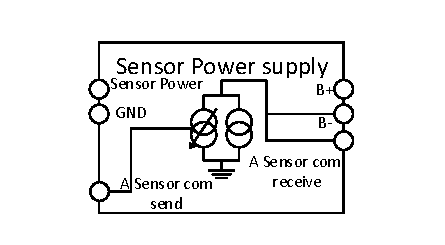
\includegraphics[scale=1]{billeder/11ProjectDescription/CDUSPS}
	\caption{Detailed CDU Sensor Power supply design.}
	\label{fig:CDUSPS}
	\end{minipage}
	\hspace{0.5cm}
	\begin{minipage}[b]{0.45\linewidth}
	\centering
	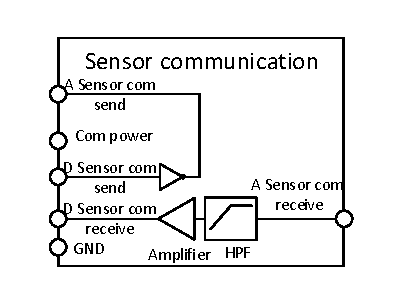
\includegraphics[scale=1]{billeder/11ProjectDescription/CDUSC}
	\caption{Detailed CDU Sensor communication design.}
	\label{fig:CDUSC}
	\end{minipage}
\end{figure}
The analog signal is extracted by the power supply block of the sensor node seen on figure \ref{fig:SN_PS_FIGURE}. The analog level signal is converted to digital levels by the communication block of the sensor node seen on figure \ref{fig:SN_com_fig}. When responding the communication block of the sensor node converts digital levels to analog levels which are transferred to the bus. The sensor communcation block of the CDU (figure \ref{fig:CDUSC}) converts the analog levels from the bus to digital levels. 
\begin{figure}[H]
	\begin{minipage}[b]{0.45\linewidth}
	\centering
	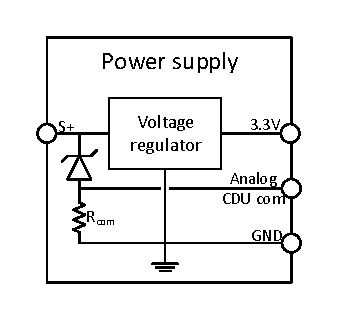
\includegraphics[width=0.8\textwidth]{billeder/11ProjectDescription/powersupply_detailed_sn}
	\caption{Sensor node power supply block}
	\label{fig:SN_PS_FIGURE}
	\end{minipage}
	\begin{minipage}[b]{0.45\linewidth}
	\centering
	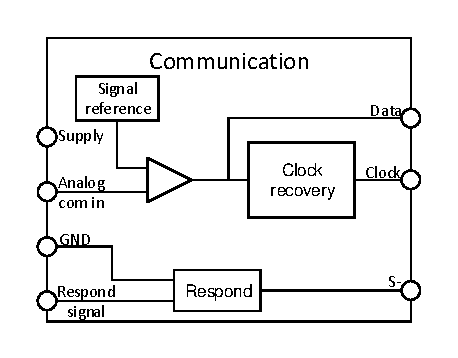
\includegraphics[width=1\textwidth]{billeder/11ProjectDescription/communication_sn}
	\caption{Sensor node communication block}
	\label{fig:SN_com_fig}
	\end{minipage}
\end{figure} 
\section{Tests}
